\documentclass{beamer}
\mode<presentation>
\usepackage{amsmath}
\usepackage{amssymb}
%\usepackage{advdate}
\usepackage{graphicx}
\graphicspath{{../figs/}}
\usepackage{adjustbox}
\usepackage{subcaption}
\usepackage{enumitem}
\usepackage{multicol}
\usepackage{mathtools}
\usepackage{listings}
\usepackage{url}
\def\UrlBreaks{\do\/\do-}
\usetheme{Boadilla}
\usecolortheme{lily}
\setbeamertemplate{footline}
{
  \leavevmode%
  \hbox{%
  \begin{beamercolorbox}[wd=\paperwidth,ht=2.25ex,dp=1ex,right]{author in head/foot}%
    \insertframenumber{} / \inserttotalframenumber\hspace*{2ex} 
  \end{beamercolorbox}}%
  \vskip0pt%
}
\setbeamertemplate{navigation symbols}{}
\let\solution\relax
\usepackage{gvv}
\lstset{
%language=C,
frame=single, 
breaklines=true,
columns=fullflexible
}

\numberwithin{equation}{section}


\title{2.10.49}
\author{EE25BTECH11020 - Darsh Pankaj Gajare}
\begin{document}
\maketitle
% \newpage
% \bigskip
Question:\\
The unit vector which is orthogonal to the vector $3\hat{i}+2\hat{j} +6\hat{k}$ and is coplanar with vectors $2\hat{i}+\hat{j}+\hat{k}$ and $\hat{i}-\hat{j}+\hat{k}$ is
\begin{multicols}{4}
	\begin{enumerate}[label=(\Alph*)]
\item $ \frac{2 \hat{i} - 6 \hat{j} + \hat{k}}{\sqrt{41}}$
\item $\frac{2\hat{i}-3\hat{j}}{\sqrt{13}}$
\item $\frac{3\hat{i}-\hat{k}}{\sqrt{10}}$
\item $\frac{4\hat{i}+3\hat{j}-3\hat{k}}{\sqrt{34}}$
\end{enumerate}
\end{multicols}
\textbf{Solution:}
Given:
\begin{table}[H]
	\centering
	\label{}
	\caption{Given data}
	\begin{tabular}{|c|c|}
\hline
\textbf{Name} & \textbf{Value} \\
\hline
Circle & $\vec{x}^\top\vec{x} - a^2 = 0$ \\
\hline
Line & $\vec{x} = \myvec{\tfrac{a}{\sqrt{2}} \\ 0} + \kappa\myvec{0 \\ 1}$ \\
\hline
\end{tabular}

\end{table}
Assume Equation of plane through $A,B$.
\begin{align}
\vec{n}^\top\vec{x}=1
\end{align}
\begin{align}
\vec{n}^\top\vec{A}=1
\end{align}
\begin{align}
\vec{n}^\top\vec{B}=1
\end{align}
\begin{align}
\myvec{2 & 1 & 1 \\ 1 & -1 & 1} n = 1
\end{align}
Augmented matrix,
\begin{align}
\augvec{3}{1}{2 & 1 & 1 & 1 \\ 1 & -1 & 1 & 1}.
\end{align}
$R_1=R_1-R_2$
\begin{align}
    \augvec{3}{1}{1 & 2 & 0 & 0\\1&-1&1&1}
\end{align}
$R_2=R_2-R_1$
\begin{align}
    \augvec{3}{1}{1&2&0&0\\0&-3&1&1}
\end{align}
Let parametric constant be $\lambda$
\begin{align}
n = \myvec{-2\lambda\\\lambda\\1+3\lambda}
\end{align}
\begin{align}
\vec{n}^\top\vec{P}=1
\end{align}
\begin{align}
\vec{C}^\top\vec{P}=0
\end{align}
\begin{align}
\myvec{-2\lambda & \lambda & 1+3\lambda \\ 3 & 2 & 6}\vec{P} = \myvec{1\\0}.
\end{align}
Augmented matrix,
\begin{align}
\augvec{3}{1}{-2\lambda & \lambda & 1+3\lambda & 1 \\ 3 & 2 & 6 & 0}.
\end{align}
Row operations:
$R_1=R_1-\frac{\lambda}{2}R_2$
\begin{align}
\augvec{3}{1}{-3.5\lambda & 0 & 1& 1 \\ 3 & 2 & 6 & 0}.
\end{align}
$R_2=R_2-6R_1$
\begin{align}
\augvec{3}{1}{-3.5\lambda & 0 & 1& 1 \\ 3+21\lambda & 2 & 0 & -6}.
\end{align}
\begin{align}
-3.5\lambda x+z=1\implies z=1+3.5\lambda x
\end{align}
\begin{align}
	\brak{3+21\lambda}x+2y=-6\implies y=-3-\frac{x}{2}\brak{3+21\lambda}
\end{align}
Let $x$ =$\mu$ a parameter
\begin{align}
\vec{P} = \myvec{\mu\\-3-\frac{\mu}{2}\brak{3+21\lambda}\\1+3.5\lambda\mu} =\myvec{0\\-3\\1}+\frac{\mu}{2}\myvec{2\\-3\\0}+7\lambda\frac{\mu}{2}\myvec{0\\-3\\1} .
\end{align}
Taking $\mu=0$ we get,
\begin{align}
	\vec{P}=\pm \myvec{0\\-3\\1}
\end{align}
Normalizing,
\begin{align}
\vec{P} = \pm \frac{1}{\sqrt{10}}\myvec{0\\-3\\1}
\end{align}\begin{figure}[H]
	\centering
	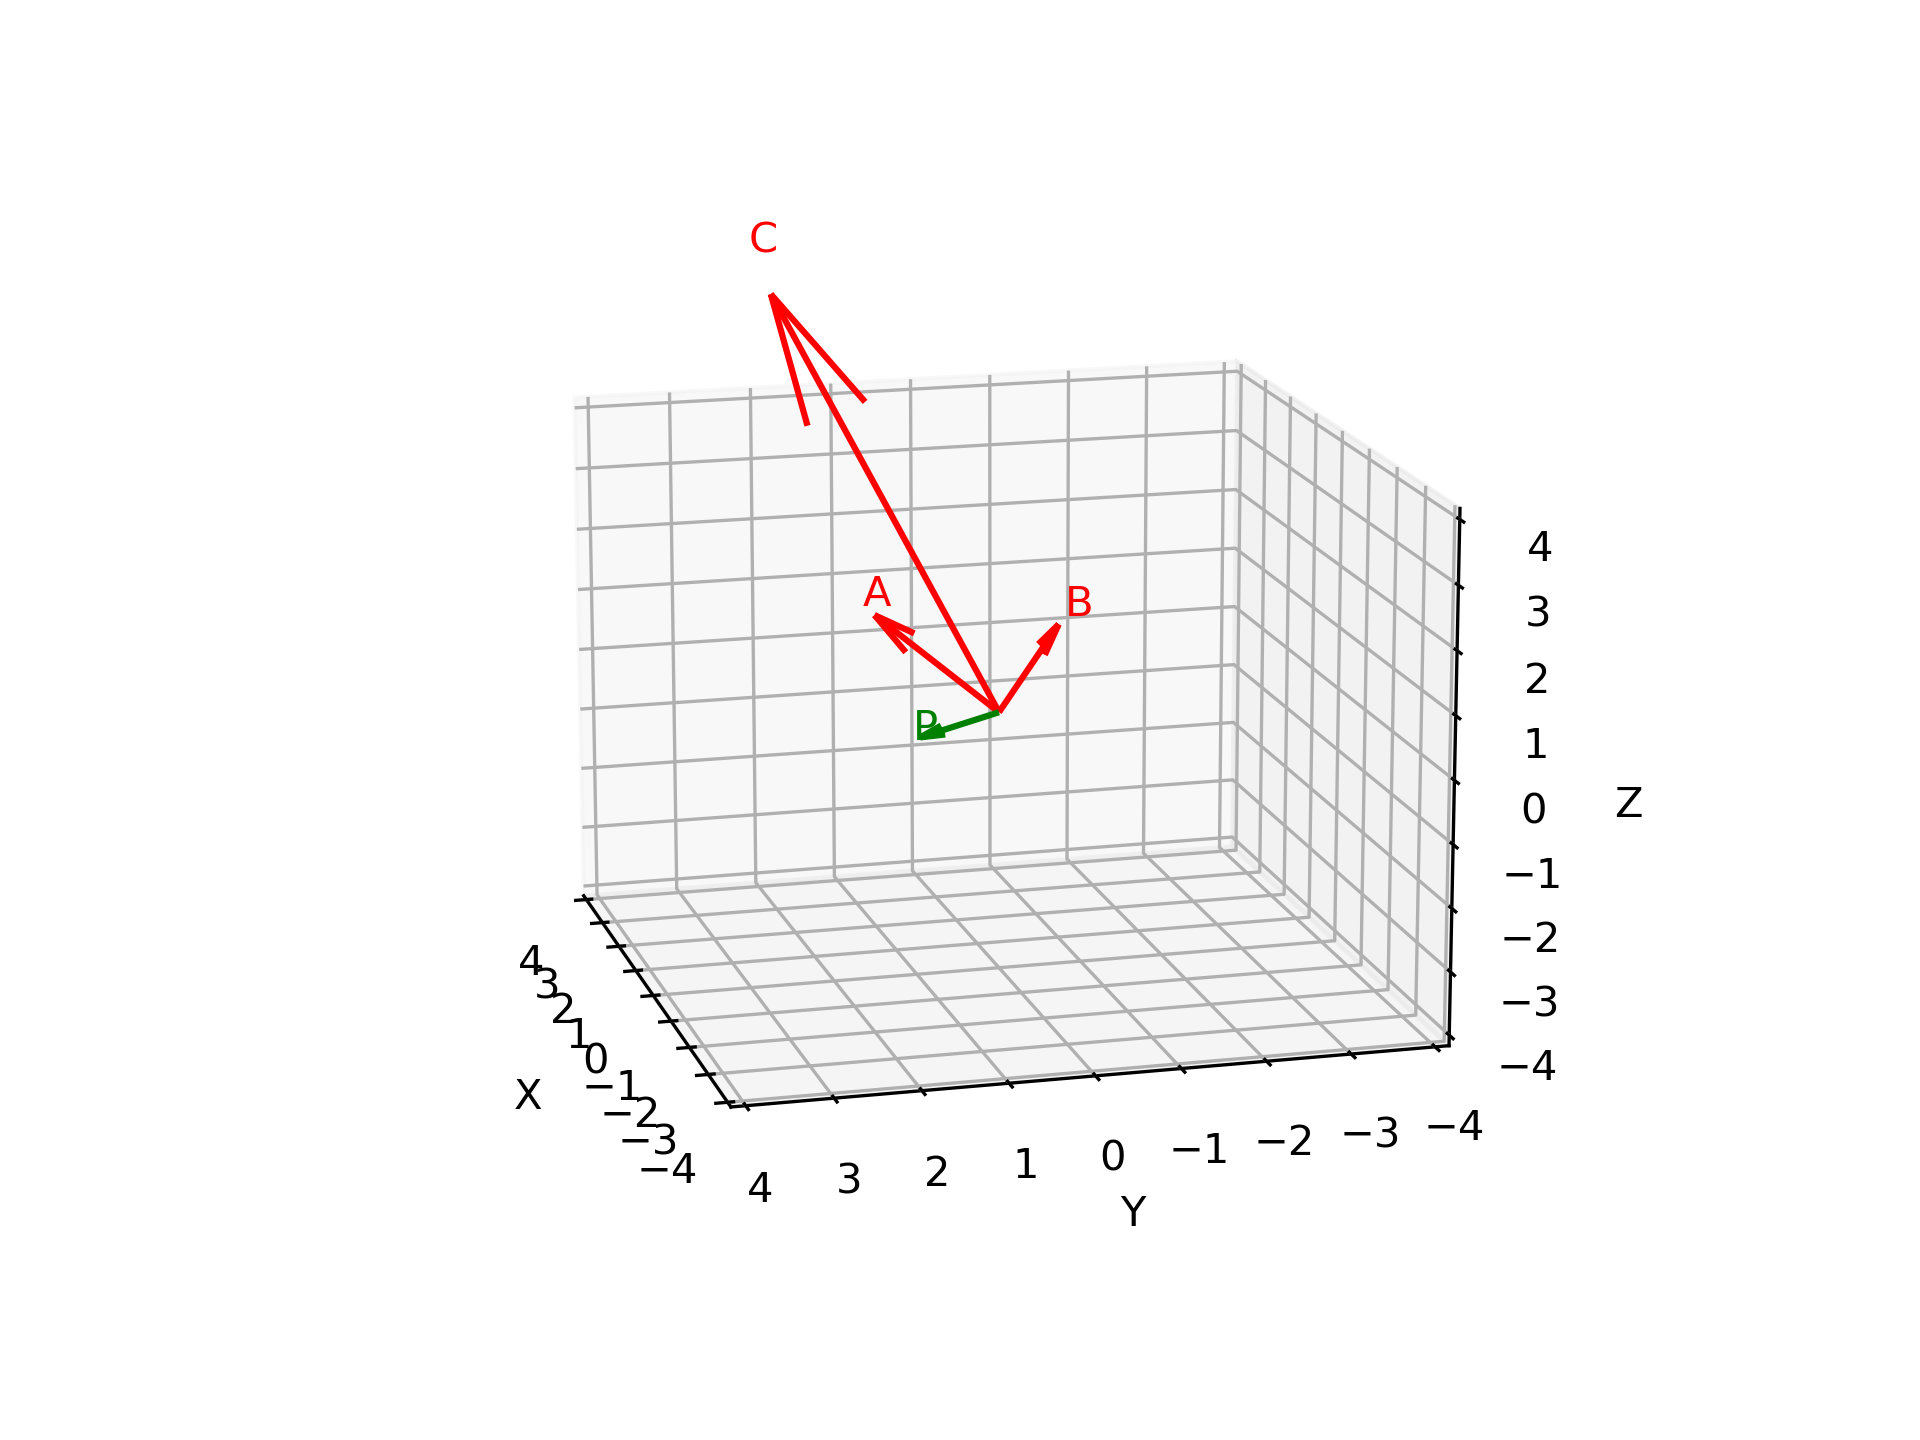
\includegraphics[scale=0.5]{img}
	\caption*{Plot using C functions}
	\label{img}
\end{figure}
\begin{figure}[H]
	\centering
	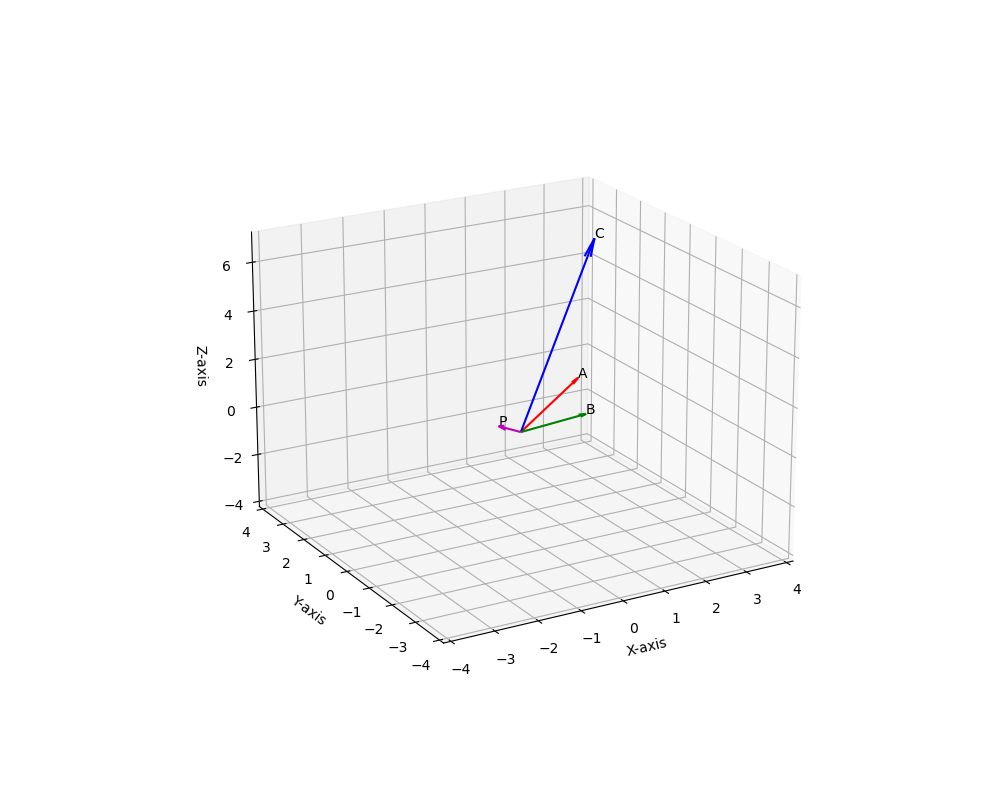
\includegraphics[scale=0.25]{fig}
	\caption*{Plot using Python}
	\label{fig}
\end{figure}
\end{document}
